\section{TÍNH ĐƠN ĐIỆU VÀ CỰC TRỊ CỦA HÀM SỐ}
\subsection{LÝ THUYẾT CẦN NHỚ}
\subsubsection{Tính đơn điệu của hàm số}
\begin{enumerate}[\iconMT]
	\item \indam{Định nghĩa:} Cho hàm số $y=f(x)$ xác định trên $K$ ($K$ là khoảng, đoạn hoặc nửa khoảng). \\
\begin{minipage}[b]{8cm}
\begin{khung4}{Ghi nhớ 1}
	Hàm số đồng biến trên $K$ nếu
	$$\forall x_1,\,x_2 \in K\colon x_1<x_2 \Rightarrow f(x_1)<f(x_2)$$
	\centerline{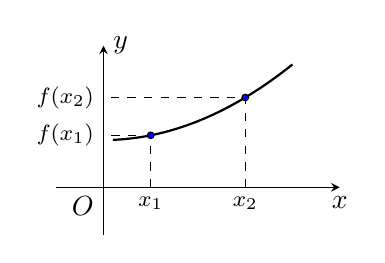
\begin{tikzpicture}[>=stealth,scale=0.6]
		\draw[->] (-1,0)--(0,0)%
		node[below left]{$O$}--(5,0) node[below]{$x$};
		\draw[->] (0,-1) --(0,3) node[right]{$y$};
		\draw [black,thick, domain=0.2:4, samples=100] %
		plot (\x, {0.1*(\x)^2+1});
		\draw [dashed] (1,0)node[below]{\footnotesize$x_1$} --(1,1.1)--(0,1.1)node[left]{\footnotesize$f(x_1)$};
		\draw [dashed] (3,0)node[below]{\footnotesize$x_2$} --(3,1.9)--(0,1.9)node[left]{\footnotesize$f(x_2)$};
		\draw[fill=blue] (1,1.1) circle(2pt);
		\draw[fill=blue] (3,1.9) circle(2pt);
	\end{tikzpicture}}\\
Trên $K$, đồ thị là một "\textbf{đường đi lên}" khi xét từ trái sang phải.
\end{khung4}
\end{minipage}\hspace{0.5cm}
\begin{minipage}[b]{8cm}
\begin{khung4}{Ghi nhớ 2}
		Hàm số nghịch biến trên $K$ nếu
		$$\forall x_1,\,x_2 \in K\colon x_1<x_2 \Rightarrow f(x_1)>f(x_2)$$
		\centerline{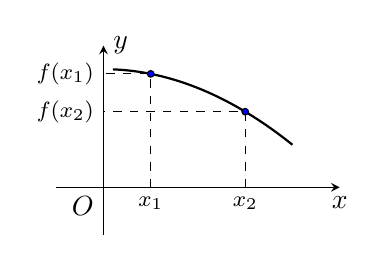
\begin{tikzpicture}[>=stealth,scale=0.6]
			\draw[->] (-1,0)--(0,0)%
			node[below left]{$O$}--(5,0) node[below]{$x$};
			\draw[->] (0,-1) --(0,3) node[right]{$y$};
			\draw [thick, domain=0.2:4, samples=100] %
			plot (\x, {-0.1*(\x)^2+2.5});
			\draw [dashed] (1,0)node[below]{\footnotesize$x_1$} --(1,2.4)--(0,2.4)node[left]{\footnotesize$f(x_1)$};
			\draw [dashed] (3,0)node[below]{\footnotesize$x_2$} --(3,1.6)--(0,1.6)node[left]{\footnotesize$f(x_2)$};
			\draw[fill=blue] (1,2.4) circle(2pt);
			\draw[fill=blue] (3,1.6) circle(2pt);
		\end{tikzpicture}}\\
	Trên $K$, đồ thị là một "\textbf{đường đi xuống}" khi xét từ trái sang phải.
\end{khung4}
\end{minipage}
	\item \indam{Liên hệ giữa đạo hàm và tính đơn điệu:}
	Cho hàm số $y=f(x)$ có đạo hàm trên khoảng $(a;b)$.
	\begin{boxdn}
	\begin{itemize}
		\item [$\bullet$] Nếu $y'\ge 0$, $\forall x \in (a;b)$ và dấu bằng chỉ xảy ra tại hữu hạn điểm thì hàm số $y=f(x)$ đồng biến trên $(a;b)$.
		\item [$\bullet$] Nếu $y'\le 0$, $\forall x \in (a;b)$ và dấu bằng chỉ xảy ra tại hữu hạn điểm thì hàm số  $y=f(x)$ nghịch biến trên $(a;b)$.
	\end{itemize}
	\end{boxdn}
\end{enumerate}
\subsubsection{Cực trị của hàm số}
\begin{enumerate}[\iconMT]
	\item \indam{Định nghĩa:} Cho hàm số $y=f(x)$ xác định và liên tục trên khoảng $(a ; b)$ ( $a$ có thể là $-\infty, b$ có thể là $+\infty)$ và điểm $x_0 \in(a ; b)$.
	\begin{boxdn}
	\begin{itemize}
		\item [$\bullet$] Nếu tồn tại số $h>0$ sao cho $f(x)<f\left(x_0\right)$ với mọi $x \in\left(x_0-h ; x_0+h\right) \subset(a ; b)$ và $x \neq x_0$ thì ta nói hàm số $f(x)$ đạt cực đại tại $x_0$.
		\item [$\bullet$] Nếu tồn tại số $h>0$ sao cho $f(x)>f\left(x_0\right)$ với mọi $x \in\left(x_0-h ; x_0+h\right) \subset(a ; b)$ và $x \neq x_0$ thì ta nói hàm số $f(x)$ đạt cực tiểu tại $x_0$.
	\end{itemize}
	\end{boxdn}
	\item \indam{Định lý:} Giả sử hàm số $y=f(x)$ liên tục trên khoảng $(a ; b)$ chứa điểm $x_0$ và có đạo hàm trên các khoảng $\left(a ; x_0\right)$ và $\left(x_0 ; b\right)$. Khi đó:
	\begin{boxdn}
	\begin{itemize}
		\item [$\bullet$] Nếu $f^{\prime}(x)<0$ với mọi $x \in\left(a ; x_0\right)$ và $f^{\prime}(x)>0$ với mọi $x \in\left(x_0 ; b\right)$ thì $x_0$ là một điểm cực tiểu của hàm số $f(x)$.
		\item [$\bullet$] Nếu $f^{\prime}(x)>0$ với mọi $x \in\left(a ; x_0\right)$ và $f^{\prime}(x)<0$ với mọi $x \in\left(x_0 ; b\right)$ thì $x_0$ là một điểm cực đại của hàm số $f(x)$.
	\end{itemize}
	\end{boxdn}
	\item \indam{Các tên gọi:}\\
		\hspace*{2cm}\begin{tikzpicture}[smooth,samples=300,scale=1.15,>=stealth]
			\draw[->,>=stealth] (-2.5,0)--(2.7,0) node[below]{$x$};
			\draw[->,>=stealth] (0,-1.5)--(0,4) node[right]{$y$};
			\draw (0,0) node[above left]{$O$};
			\draw[blue,domain=-2:2,line width = 1.2pt] plot(\x,{(\x)^3-3*(\x)+1})node[right]{$y=f(x)$};
			\draw[fill=black] (1,0) circle(1pt) (1,-1) circle(2pt) (0,-1) circle(1pt) (-1,0) circle(1pt) (-1,3) circle(2pt) (0,3) circle(1pt);
			\draw[dashed] (1,0)node[above]{\small$x_2$}--(1,-1)--(0,-1)node[left]{\small$y_2$} (-1,0)node[below]{\small$x_1$}--(-1,3)--(0,3)node[right]{\small$y_1$};
			
			\draw[-,dotted] (-0.5,3.7)--(4,3.7)node[right]{$(x_1;y_1)$ là điểm cực đại của đồ thị hàm số;}; 
			\draw[->,dotted] (-0.5,3.7)--(-1,3.15);
			\node[right] at (4.5,3.1) {$\bullet$ $x_1$ là điểm cực đại của hàm số;};
			\node[right] at (4.5,2.5) {$\bullet$ $y_1$ là giá trị cực đại của hàm số.};
			
			\draw[-,dotted] (2,-1)--(2,1)--(4,1)node[right]{$(x_2;y_2)$ là điểm cực tiểu của đồ thị hàm số;}; \draw[->,dotted] (2,-1)--(1.15,-1);
			\node[right] at (4.5,0.4) {$\bullet$ $x_2$ là điểm cực tiểu của hàm số;};
			\node[right] at (4.5,-0.2) {$\bullet$ $y_2$ là giá trị cực tiểu của hàm số.};
		\end{tikzpicture}
\end{enumerate}
